\chapter*{Week 4: Functions}
\addcontentsline{toc}{chapter}{Week 4: Functions}
\setcounter{chapter}{4}
\setcounter{section}{0}

\begin{abstract}
This week you will:
\begin{enumerate}
    \item Understand switch statements
    \item Understand basic functions:
    \begin{itemize}
        \item Return types
        \item Parameter lists
        \item Function calls
    \end{itemize}
    \item Be able to identify the scope of a variable

\end{enumerate}
    
\end{abstract}

\section{Background}

\subsection{Switch Statements}
Switch statements are an easy way to make decisions in a program. We can execute different sections of our code based on the value of a character or integer variable. 
\begin{itemize}
    \item If we are building a switch statement around an \mintinline{c++}{int} variable, all of the cases must be defined using numbers. 
    \item If we are building a switch statement around a \mintinline{c++}{char} variable, all of the cases must be defined using characters. This means they must also use single quotes. 
\end{itemize}

\begin{center}
    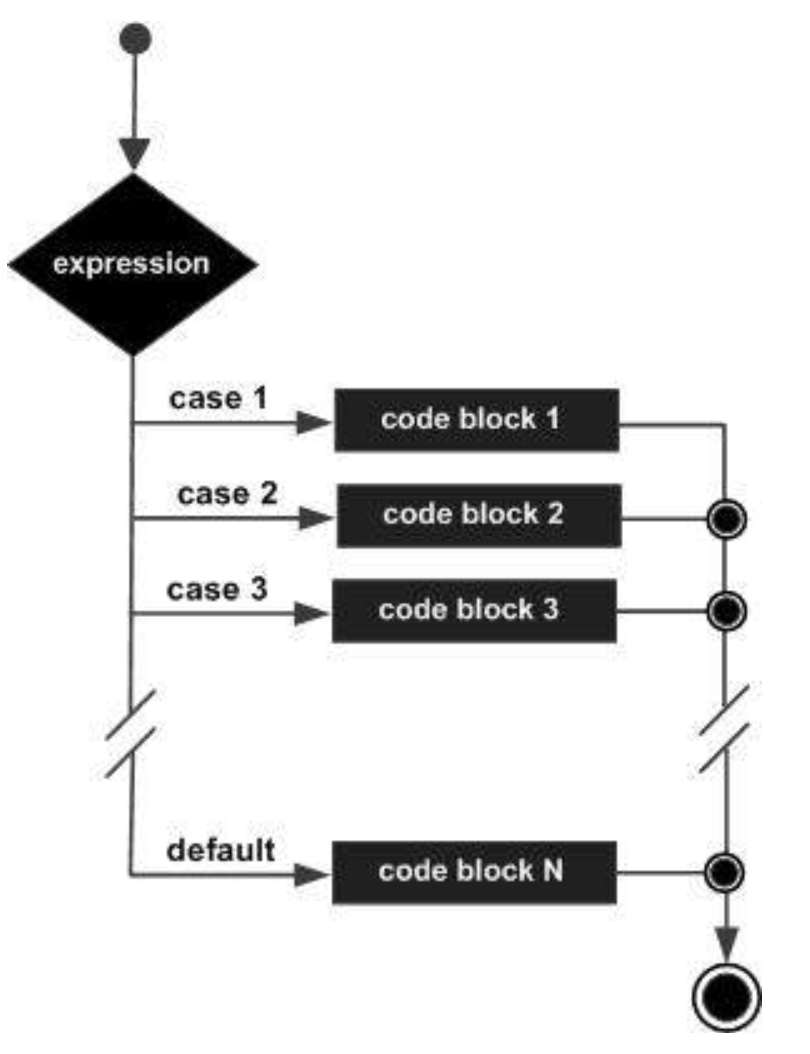
\includegraphics[width = 3in]{images/switchdiagram.png}
\end{center}

With the switch statement, the variable name is used once in the opening line. The \mintinline{c++}{case} keyword is used to provide the possible values of the variable, which is followed by a colon and a set of statements to run if the variable is equal to a corresponding value.

An example of a simple switch statement:

\begin{example}
    Switch statement syntax:
\begin{minted}{c++}
switch (n){
     case 1:
          // code to be executed if n == 1;
          break;
     case 2:
          // code to be executed if n == 2;
          break;
     default:
          // code to be executed if n doesn’t match any cases
}
\end{minted}
\end{example}

Important notes to keep in mind when using switch statements :

\begin{itemize}
    \item The expression provided in the switch should result in a constant value otherwise it would not be valid.
    \begin{itemize}
        \item \mintinline{c++}{switch(num)}
        \begin{itemize}
            \item allowed (\mintinline{c++}{num} is an integer variable)
        \end{itemize}
        \item \mintinline{c++}{switch('a')}
        \begin{itemize}
            \item allowed (takes the ASCII Value)
        \end{itemize}
        \item \mintinline{c++}{switch(a+b)}
        \begin{itemize}
            \item allowed, where \mintinline{c++}{a} and \mintinline{c++}{b} are \mintinline{c++}{int} variables, which are defined earlier
        \end{itemize}
    \end{itemize}
    \item The \mintinline{c++}{break} statement is used inside the switch to terminate a statement sequence. When a \mintinline{c++}{break} statement is reached, the switch terminates, and the flow of control jumps to the next line following the switch statement.
    \item The \mintinline{c++}{break} statement is optional. If omitted, execution will continue on into the next case. The flow of control will fall through to subsequent cases until a break is reached.
    \item The default statement is optional. Even if the switch case statement does not have a default statement, it would run without any problem.
\end{itemize}

Switch statements are a simple way to make decisions based exclusively on the equivalence of some characters or numbers. They are a simple form of \textbf{conditional statement}.

\subsection{Functions}
``Functions" in the context of math may be familiar, especially when formatted like this:
$$f(x) = x^2 + 5$$

Here we have labeled our function $f$, and it is a function of the variable $x$. You might have seen some where the functions are functions on multiple variables:

$$g(x,y) = x^2+y^3$$

Functions in computer science are similar, but we can abstract them further so they apply to more than just numbers. 

A function is a named block of code which is used to perform a particular task. The power of functions lies in the capability to perform that task anywhere in the program without requiring the programmer to repeat that code many times. This also allows us to group portions of our code around concepts, making programs more organized. You can think of a function as a mini-program.

There are two types of functions:

\begin{itemize}
    \item Library functions
    \item User-defined functions
\end{itemize}

Library functions refer to pre-existing functions that you can use but did not write yourself. In order to use a library function, you must include the library that contains the function. For example, the C++ math library provides a \mintinline{c++}{sqrt()} function to calculate the square root of a number. To use the \mintinline{c++}{sqrt()} function, you must include the cmath library at the top of your program, e.g. \mintinline{c++}{#include<cmath>}. Libraries other than the built-in C++ libraries can be found online.

C++ allows programmers to define their own functions. These are called user-defined functions. Every valid C++ program has at least one function, the \mintinline{c++}{main()} function.

We pass values to functions via parameters. In general, the parameters should be all the information needed for the function to do its work. When that work is complete, we would like to use the result in other code. The function can return one value of the specified return type. A function may also return nothing, in which case its return type is void.

Here is the syntax for a function definition:

\begin{minted}{c++}
returnType functionName(parameterList)
{
    //function body
}
\end{minted}

\begin{itemize}
    \item The \mintinline{c++}{returnType} is the data type that the function returns
    \item \textcolor{blue}{\mintinline{c++}{functionName}} is the actual name of the function
    \item \mintinline{c++}{parameterList} refers to the type, order, and number of the parameters of a function. A parameter is like a placeholder. When a function is invoked, you pass a value to the parameter. This value is referred to as actual parameter or argument. Note: this can be a list of multiple items separated by commas. 
    \item \mintinline{c++}{//function body} contains a collection of statements that define what the function does. The statements inside the function body are executed when a function is called.
\end{itemize}

This may not immediately look like the functions you have seen in math, but they are actually quite close. Here is an example of the functions above written in C++:

\begin{example}
    The function $f(x) = x^2 + 5$ written in C++:

    \begin{minted}{c++}
double f(double x){
    return (x*x+5);
}
    \end{minted}
\end{example}

\begin{example}
    The function $g(x,y) = x^2+y^3$ written in C++:

    \begin{minted}{c++}
double g(double x, double y){
    return (x*x+y*y*y);
} 
    \end{minted}
\end{example}

I used \mintinline{c++}{double} for the parameters and the return type because these functions in math would probably use decimals, but you could also use integers if you only wanted to use whole numbers. We can also use functions inside of other functions. Instead of just multiplying variables by themselves to do the exponents, we could use the \mintinline{c++}{pow} function from \mintinline{c++}{cmath}:

\begin{example}
    The function $f(x) = x^2 + 5$ written using cmath:

    \begin{minted}{c++}
#include<cmath>

double f(double x){
    return pow(x, 2)+5;
}
    \end{minted}
\end{example}

\begin{example}
    The function $g(x,y) = x^2+y^3$ written using cmath:

    \begin{minted}{c++}
#include<cmath>

double g(double x, double y){
    return pow(x, 2) + pow(y, 3);
} 
    \end{minted}
\end{example}

If you wanted to then use these functions to perform some calculations, you could use any value of $x$ and $y$. You could use constant values, or you could use variables. Here are examples of ways you could use the function:

\begin{example}
    Examples of calling the function $g(x,y)$:

    \begin{minted}{c++}
#include<cmath>
#include<iostream>

using namespace std;

double g(double x, double y){
    return pow(x, 2) + pow(y, 3);
} 

int main(){
    double firstValue = g(4.0, 5.0);
    double secondValue = g(2, 3); 
    double myX, myY;

    cout << "What value would you like for X?" << endl;
    cin >> myX;
    cout << "What value would you like for Y?" << endl;
    cin >> myY;
    cout << "The result would be " << g(myX, myY) << endl;

    return 0;
}

    \end{minted}
\end{example}

A function has its own \textbf{scope}. That means that the parameters of the function, as well as local variables declared within the function body, are not accessible outside the function. This is useful because it allows us to solve a small problem in a self-contained way. Parameter values and local variables disappear from memory when the function completes its execution. We can illustrate the order in which code executes with this example:

\begin{example}
    An example with a simple function:
\begin{minted}[xleftmargin=20pt, linenos]{c++}
#include <iostream>
using namespace std;

//funtion to add two numbers
int sum( int num_one, int num_two)
{
    int result = num_one + num_two;
    return result;
}

//main function
int main()
{
    //declare parameter value
    int parameter_var = 1;
    
    //call the function
    int sum_result = sum(parameter_var, 99);
    
    cout << "The sum is " << sum_result << endl;
    
    return 0;
}    
\end{minted}
\end{example}

The code will begin executing in the main function -- in this case, the first step is declaring a variable in line 15. When the program execution reaches line 18, the main function will pause, and the first line in the body of the \mintinline{c++}{sum()} function will begin running. After the line \mintinline{c++}{return result;} is reached, \mintinline{c++}{sum()} will stop running, and the main program will resume execution where it left off. In this case, when \mintinline{c++}{main()} resumes execution, the return value of \mintinline{c++}{sum()} will be stored in \mintinline{c++}{int sum_result}, and then the last two lines of the main function will run.

Functions can do more than just perform calculations; they can also perform operations on other variables, or they can be used to prevent yourself from copy/pasting the same code multiple times in your program. They do not even always need parameters. For example, if you wanted to write out a selection menu, you could write a function to print the menu so you do not have to type it out every time. In these cases, the parenthesis can be empty, like they are for our main functions. 

As a general note: the function names $f$ and $g$ are not very good function names. You should generally pick better (clearer) names, and you should choose a naming style to be consistent. The naming style you choose should be different from how you name variables, so it is easier to read your code.We recommend using camel case to name your functions, like so:

Examples of function names we might use: \mintinline{c++}{circleArea(), sumList(), findCapitalLetters()}


\subsection{Testing Code}
You must naturally test your code to make sure that it works correctly, and that it works correctly \textbf{all} the time. This may seem like a very difficult task, but there are several steps you can take to make sure you start correctly.

\begin{itemize}
    \item Come up with a handful of test cases to use on your program. 
    \item Consider the ways a user could use your program incorrectly. Use this to develop additional test cases.
    \item Consider extreme values, or "boundary conditions". Use these boundary conditions to develop yet more test cases.
    \item Test each part of your program independently. This is called \textit{Unit Testing}. Do you have individual functions? Test each of them. Do you have major steps in your main function? Test each of them.
\end{itemize}

Boundary conditions are significant for many complex problems, and should test the extreme limits of what your problem may be applied to. Example: Are you supposed to examine a string? What happens if that string is empty? What happens if that string is thousands of digits long? 

You should develop test cases for each boundary condition you can come up with. If there are several components to your program, you may need to identify boundary conditions for each of these components. Testing these boundary conditions of these pieces individually -- whether they are functions or just blocks of code in your main function -- is often easier than testing every independent combination of them. 

Consider a program where you have 4 functions, and each function has 3 boundary conditions. To test each boundary condition for each of the 4 functions, you would need 12 tests. If however you only tested the program as a whole, you might need to check each combination of boundary conditions, which would end up becoming $3^4 = 81$ different tests. This is part of why \textbf{unit testing} is valuable. 

As you develop extra functions, you should start by using your \mintinline{c++}{main} function to test these functions. There will be 3 different types of test cases you should be expected to write depending on the return type of the function. Listed below is how we expect you to test different types of functions. The process will be different for if you are testing a \mintinline{c++}{void} function, non-void functions that return an \mintinline{c++}{int} or \mintinline{c++}{bool}, and non-void functions that return a \mintinline{c++}{double}.

\subsubsection{Testing Void Functions}

For void functions that have printed output (i.e. functions that use cout to print to the terminal), call the testing function in the main function. Your tests should include the expected output in comments. For these functions you will want to make sure that all expected outputs are successfully printed.

See the example code below:

\begin{example}
    This is testing a function that prints whether a grade is passing or not. 
    \begin{minted}{c++}
    void checkGrade(char grade){
        switch(grade){
            case 'a':
            case 'b':
            case 'c':
                cout << "You passed!" << endl;
                break;
            case 'd':
                cout << "You did not pass, but you were close." << endl;
                break;
            case 'f':
                cout << "You failed." << endl;
                break;
            default:
                cout << "That is not a valid grade." << endl;
        }
    }        

    int main(){
        checkGrade('b'); //Should output "You passed!"
        checkGrade('d'); //Should output "You did not pass, but you were close."
        checkGrade('f'); //Should output "You failed."
        checkGrade('m'); //Should output "That is not a valid grade."
    }
    \end{minted}

\end{example}

\subsubsection{Testing Integer/Boolean Functions}

For non-void functions that return a \mintinline{c++}{bool} or \mintinline{c++}{int}, use an \mintinline{c++}{assert} statement from the \mintinline{c++}{cassert} header (\mintinline{c++}{#include <cassert>}) with a conditional expression.

Assert tests contain a conditional expression which will be true unless there is a bug in the program. If the conditional expression evaluates to false, then your program will terminate and show an error message.

For immediate purposes, functions that return a \mintinline{c++}{bool} or \mintinline{c++}{int} can be compared to a specific value using the equality operator \mintinline{c++}{==}.

Your test will look something like this:

\mintinline{c++}{assert(<function call> == <value to compare to>);}

\begin{itemize}
    \item \mintinline{c++}{<function call>} is where you will call the function you want to test with its function parameters.
    \item \mintinline{c++}{<value to compare to>} is the value you expect the function to return.
    \item \mintinline{c++}{==} is the equality operator, and it compares the equality of both sides of itself.
\end{itemize}

See the sample code below:

\begin{example}
    The below code shows examples of how to test integer functions with a simple addition function:
    \begin{minted}{c++}
    #include <iostream>
    #include <cassert>
    using namespace std;
    
    int addInts(int num1, int num2)
    {
        // add num1 and num2 before returning
        return num1 + num2;
    }
    
    int main()
    {
        // test 1 for addInts
        assert(addInts(5, 6) == 11);
        // test 2 for addInts
        assert(addInts(10, 10) == 20);
    }
    \end{minted}
\end{example}

\subsubsection{Testing Double Functions}
For non-void functions that return a double, use an \mintinline{c++}{assert} statement from the \mintinline{c++}{cassert} header (\mintinline{c++}{#include <cassert>}) with a conditional expression and include the following function in your program:

\begin{example}
    This is a required function to successfully test Double functions in C++:
    \begin{minted}{c++}
        /**
         * doublesEqual will test if two doubles are equal to each 
         * other within two decimal places.
         */
        bool doublesEqual(double a, double b, const double epsilon = 1e-2)
        {
            double c = a - b;
            return c < epsilon && -c < epsilon;
        }
    \end{minted}
\end{example}

Because the \mintinline{c++}{double} type holds so much precision, it will be hard to compare the equality of a function that returns a \mintinline{c++}{double} with another \mintinline{c++}{double} value. To overcome this challenge, we can compare \mintinline{c++}{double} values within a certain range of precision or decimal places. The function above compares the equality of two values \mintinline{c++}{a} and \mintinline{c++}{b} up to two decimal places. This function returns \mintinline{c++}{true} if the values \mintinline{c++}{a} and \mintinline{c++}{b} are equal with each other up to two decimal places.

You will be expected to use this function in conjunction with assert statements to test functions that return the type double.

Your test will look something like this:

\mintinline{c++}{assert(doublesEqual(<function call>, <value to compare to>));}

\begin{itemize}
    \item \mintinline{c++}{<function call>} is where you will call the function you want to test with its function parameters
    \item \mintinline{c++}{<value to compare to>} is the double value you expect the function to return.
\end{itemize}

See the sample code below:

\begin{example}
    This is code to test a function that finds the reciprocal of a value (i.e., divides 1 by that number).
    \begin{minted}{c++}
        #include <iostream>
        #include <cassert>
        using namespace std;
        /**
         * doublesEqual will test if two doubles are equal to each other within 
         * two decimal places.
         */
        bool doublesEqual(double a, double b, const double epsilon = 1e-2)
        {
            double c = a - b;
            return c < epsilon && -c < epsilon;
        }
        /**
         * reciprocal returns the value of 1 divided by the number 
         * passed into the function.
         */
        double reciprocal(int num)
        {
            return 1.0 / num;
        }
        int main()
        {
            // test 1 for reciprocal
            assert(doublesEqual(reciprocal(6), 0.16));
            // test 2 for reciprocal
            assert(doublesEqual(reciprocal(12), 0.083));
        }
    \end{minted}
\end{example}

\subsubsection{General Testing Tips}
You will certainly come to a time in your coding career when your code does not work, and you just cannot figure out \textit{why}.

In these times, there are a few possible options. First, your algorithm may be incorrect. If that is the case no amount of code testing will help you, and you will need to go back and think through how to solve the problem. If your algorithm is correct but your code is not, here are three tips:
\begin{enumerate}
    \item If your code does not compile, start commenting out sections of your code. Keep going until it compiles, even if you have to go all the way back to an empty main function. Then, you can uncomment sections of your code until it fails to compile again. This will help you pinpoint \textit{where} the issue is in your code, and once you know where it is you will be able to see \textit{what} it is. 
    \item If your code compiles but has unexpected runtime errors, add output statements periodically throughout your code. When your program fails, you will know where your code stopped running based on which output statements failed to print.
    \item If your code compiles and runs completely but the output is incorrect, go back through your code and print out the significant variables at each step in your code. You can then compare this to the test cases you worked out by hand and see where the code output differs from your algorithm.
\end{enumerate}

\section{PreQuiz}

\begin{problem}
    Select True or False:
    \begin{enumerate}[label=\Alph*)]
        \item \textbf{T/F:} When writing switch statements in C++ you must include a default case, otherwise your switch statement is not valid.
        \item \textbf{T/F:} Switch statements can be built on integers, floats, and characters.
        \item \textbf{T/F:} There is no difference between an if/else-if/else-if chain and an if/if/if chain in C++.
    \end{enumerate}
\end{problem}

\begin{problem}
    Given two conditions, \mintinline{c++}{cond1} and \mintinline{c++}{cond2}, the expression if \mintinline{c++}{(cond1 && cond2)} will evaluate to true only if \textunderscore \textunderscore \textunderscore \textunderscore \textunderscore \mintinline{c++}{cond1} and \mintinline{c++}{cond2} are true. On the other hand, the expression if \mintinline{c++}{(cond1 || cond2)} will evaluate to true if \textunderscore \textunderscore \textunderscore \textunderscore \textunderscore \mintinline{c++}{cond1} or \mintinline{c++}{cond2} is true.
\end{problem}

\begin{problem}
    How can you write a switch statement where multiple cases will execute the same block of code? Provide an example.
\end{problem}

\vspace{5cm}

\begin{problem}
    Fill in the blank(s) for the code below:
    \begin{minted}{c++}
    int choice;
    cout << "Help our adventurer discover what to do next! Enter 1, 2, or 3." << endl;
    ______ >> choice;

    switch(____________){
        case ________:
            cout << "You found a hidden treasure!" << endl;
            break;
        case 2:
            cout << "You discovered a secret passage!" << endl;
            ___________
        case 3:
            cout << "You found a mystical artifact!" << endl;
            break;
        ________:
            cout << "That's not a valid case. Please try again." << endl;
    }
    \end{minted}
\end{problem}



\section{Recitation}

\subsection{Spot The Error}

\begin{multipart}
Below is code that asks the user for the day of the week as a number (Monday is 1, Sunday is 7) and then prints a corresponding statement. Identify the error(s):
\begin{minted}{c++}
    int day;
    cout << "What number day of the week is it?" << endl;
    cin >> day;
    switch (day) {
      case '6':
        cout << "Today is Saturday";
        break;
      case 7:
        cout << "Today is Sunday";
        
      default:
        cout << "Looking forward to the Weekend";
    }
\end{minted}

\end{multipart}

\begin{multipart}
    Below is code with the same goal as the previous question, but different error(s). Identify the error(s):
    \begin{minted}{c++}
    int day = 4;
    switch (day) 
      case 6:
        cout << "Today is Saturday";
        break;
      case 7:
        cout << "Today is Sunday";
        break;
      default
        cout << "Looking forward to the Weekend";
        
    \end{minted}
\end{multipart}

\begin{multipart}
    The code below is meant to determine if an angle is acute, obtuse, or right. Spot the error(s):
    \begin{minted}{c++}
    #include <iostream>
    using namespace std;
    
    int main()
    {
        int angle =40;
        if (x<90) { 
            cout<<"It is an acute angle." ;
        }
        else if(x=90) {
            cout<<"It is a right angle.";
        }
        els{
            cout<<"It is an obtuse angle.";
        }
    }
    \end{minted}
\end{multipart}

\begin{multipart}
    The code below implements an exclusive OR logical operation, which means that only one of the conditions may be true. Spot the error(s):
    \begin{minted}{c++}
    // This program implements XOR
    #include iostream
    using namespace std;
    
    //Set the variable value to 1 when x or y is 1
    int main(){
        int x = 1,y=0,value;
        
        if (x == 1){ 
            if(y==0)
            value = 1; 
    
            else
            y == 0; 
         
        if(x==0){ 
            if(y==0)
            value = 0; 
    
            else
            value = 1;
        }
        
        cout < value < endl;
        return 0;
    }
    \end{minted}
\end{multipart}

\subsection{Final Velocity of a Rocket}

Write a C++ program that will calculate the final velocity of a rocket after 20 seconds. The program will ask the user for the initial velocity (m/s) and the fuel type (A, B, C). The rate of acceleration will depend on the type of fuel and the initial velocity.

\begin{itemize}
    \item If initial velocity is less than 10, then the acceleration rate for each fuel type is as follows
    \begin{itemize}
        \item Fuel type A $\rightarrow$ 5 (m/s) per second
        \item Fuel type B $\rightarrow$ 10 (m/s) per second
        \item Fuel type C $\rightarrow$ 20 (m/s) per second
    \end{itemize}
   \item If initial velocity is greater than or equal to 10 and less than or equal to 40, then the acceleration rate
   for each fuel type is as follows
   \begin{itemize}
        \item Fuel type A $\rightarrow$ 6 (m/s) per second
        \item Fuel type B $\rightarrow$ 12 (m/s) per second
        \item Fuel type C $\rightarrow$ 24 (m/s) per second
   \end{itemize}
    \item If initial velocity is greater than 40, then the acceleration rate for each fuel type is as follows
    \begin{itemize}
        \item Fuel type A $\rightarrow$ 3 (m/s) per second
        \item Fuel type B $\rightarrow$ 6 (m/s) per second
        \item Fuel type C $\rightarrow$ 9 (m/s) per second 
    \end{itemize}
\end{itemize}

Below are some sample runs. User input is shown in bold. 

\begin{sample}
    Enter the initial velocity:
    
    \textbf{70}
    
    Enter the fuel type:
    
    \textbf{C}
    
    The final speed is 250 m/s.
\end{sample}

\begin{sample}
    Enter the initial velocity:
    
    \textbf{5}
    
    Enter the fuel type:
    
    \textbf{A}
    
    The final velocity is 105 m/s.
\end{sample}

\newpage

\begin{multipart}
    Write out the steps you would use to solve this problem by hand as pseudocode. 
\end{multipart}

\vspace{10cm}

\begin{multipart}
    Pick possible inputs for your program. Follow the steps you wrote for these values to find your result, and verify it.
\end{multipart}

\vspace{3.5cm}

\begin{multipart}
     Identify two possible values that are ``boundaries" in this problem that you will have to test. What should happen for these values?
\end{multipart}

\vspace{3.5cm}

\begin{multipart}
    Translate your pseudocode into a c++ program to solve the above code.
\end{multipart}


\section{Homework}

\subsection{Car switch}

Write a program that accepts a single character representing an automobile manufacturing company as input from the user. Then, the program should print out the text for the appropriate company

\begin{itemize}
\item Your program prompts the user with “Enter the first letter of the company: ”, which asks for a character input. 
\item The input must be case sensitive, e.g., if the user enters ‘b’ instead of ‘B’, the output should be invalid and not “BMW”.
    \item Your program prints output according to the following:
    \begin{itemize}
        \item If the input is ‘B’, print “BMW”
        \item If the input is ‘V’, print “Volkswagen”
        \item If the input is ‘H’, print “Honda”
        \item If the input is ‘T’, print “Tesla”
        \item Any input value that is not ‘B’, ‘V’, ‘H’, or ‘T’ should print “Invalid”
    \end{itemize}
\end{itemize}



\textbf{Note:} Code should NOT contain any  if-else statements and should only utilize Switch Statements


\begin{sample}
Enter the first letter of the company:

 \textcolor{red}{B}
 
Automobile manufacturer chosen: BMW


\end{sample}

\begin{sample}
Enter the first letter of the company:

 \textcolor{red}{V}
 
Automobile manufacturer chosen: Volkswagen


\end{sample}

\begin{sample}
Enter the first letter of the company:

 \textcolor{red}{A}
 
Automobile manufacturer chosen: Invalid

\end{sample}
\begin{sample}
Enter the first letter of the company:

 \textcolor{red}{T}
 
Automobile manufacturer chosen: Tesla

\end{sample}

\subsection{Instrument Price}

You want to learn to play an instrument, but you need to know how much it will cost to buy it. The music store has the following table on their website:


\begin{table}[H]
    \centering
       \begin{tabular}{|c|c|c|}
    \hline
    \textbf{Category} & \textbf{Instrument} & \textbf{Price} \\
    \hline
    Brass & Trumpet & \$570 \\
                           & Trombone & \$500 \\
    \hline
    Woodwind & Flute & \$425 \\
                              & Saxophone & \$225 \\
    \hline
    Percussion & Snare Drum & \$275 \\
                                & Cymbals & \$350 \\
    \hline
    \end{tabular}

\end{table}

Write a menu-driven program that asks the user to input an instrument category and then an instrument. The program should give the user the price.

The user should input an integer in the range of the choices you give them (for example, a user cannot input 3 if you only have 2 choices). If the user inputs the correct range, the program should be prompted for the next set of choices. Once they make the final selection, the total should be printed to them as an integer with proper formatting, as shown in the sample run. \\

\textbf{Note:} Code should NOT contain any  if-else statements and should only utilize Switch Statements


\begin{sample}
Select a category: (1)Brass (2)Woodwind (3)Percussion

 \textcolor{red}{1}
 
Select an instrument: (1)Trumpet (2)Trombone

 \textcolor{red}{2}
 
Your instrument will be \$500

\end{sample}

\begin{sample}
Select a category: (1)Brass (2)Woodwind (3)Percussion

 \textcolor{red}{3}
 
Select an instrument: (1)Snare Drum (2)Cymbals

 \textcolor{red}{2}
 
Your instrument will be \$350

\end{sample}

\begin{sample}
Select a category: (1)Brass (2)Woodwind (3)Percussion

 \textcolor{red}{5}
 
Please enter a valid input.

\end{sample}
\begin{sample}
Select a category: (1)Brass (2)Woodwind (3)Percussion

 \textcolor{red}{2}
 
 
Select an instrument: (1)Flute (2)Saxophone

 \textcolor{red}{1}
 
Your instrument will be \$425.


\end{sample}

\subsection{Movie Night}

You are preparing a movie night with your friends. Create a C++ program that helps you determine which movie to select. \\

Based on the given table, you, as the programmer, should give step-by-step choices to the user to proceed further and make a movie selection. Once the user has selected the movie, the program should display a message: ``You have selected the movie: <movie title>" where ``<movie title>" is the movie the user has selected. \\

Additionally, ensure that the user's input is present in the range of choices. If the user inputs an invalid option, print ``Please enter a valid input" and terminate the program. 

\begin{table}[h!]
\centering
\begin{tabular}{|c|l|l|}
\hline
\textbf{Genre}        & \textbf{Directors}         & \textbf{Movies}                 \\ \hline
\multirow{6}{*}{(1) Animation} & \multirow{2}{*}{(1) Pete Docter} & (1) Monsters, Inc.            \\ \cline{3-3} 
                   &                              & (2) Inside Out      \\ \cline{2-3} 
                   & \multirow{2}{*}{(2) 	Brad Bird}     & (1) The Incredibles          \\ \cline{3-3} 
                   &                              & (2) Ratatouille                \\ \cline{2-3} 
                   & \multirow{2}{*}{(3) Andrew Stanton} & (1) Finding Nemo             \\ \cline{3-3} 
                   &                              & (2) WALL-E      \\ \hline
\multirow{6}{*}{(2) Adventure} & \multirow{2}{*}{(1) Steven Spielberg}       & (1) E.T. the Extra-Terrestrial \\ \cline{3-3} 
                   &                              & (2) The BFG           \\ \cline{2-3} 
                   & \multirow{2}{*}{(2) 	Jon Favreau}      & (1) The Jungle Book (2016)      \\ \cline{3-3} 
                   &                              & (2) Elf              \\ \cline{2-3} 
                   & \multirow{2}{*}{(3) Robert Zemeckis}     & (1) Back to the Future          \\ \cline{3-3} 
                   &                              & (2) Who Framed Roger Rabbit                 \\ \hline
\end{tabular}
\end{table}


\begin{sample}
Select the genre: (1) Animation (2) Adventure

\textcolor{red}{1}

Select the director: (1) Pete Docter (2) Brad Bird (3) Andrew Stanton

\textcolor{red}{1}

Select the movie: (1) Monsters, Inc. (2) Inside Out

\textcolor{red}{1}

You have reserved the movie: Monsters, Inc.
\end{sample}

\begin{sample}
Select the genre: (1) Animation (2) Adventure

\textcolor{red}{2}

Select the director: (1) Steven Spielberg (2) Jon Favreau (3) Robert Zemeckis

\textcolor{red}{1}

Select the movie: (1) E.T. the Extra-Terrestrial (2) The BFG

\textcolor{red}{1}

You have reserved the movie: E.T. the Extra-Terrestrial

\end{sample}

\begin{sample}
Select the genre: (1) Animation (2) Adventure

\textcolor{red}{4}

 Please enter a valid input
\end{sample}

\begin{sample}
Select the genre: (1) Animation (2) Adventure

\textcolor{red}{2}

Select the director: (1) Steven Spielberg (2) Jon Favreau (3) Robert Zemeckis

\textcolor{red}{2}

Select the movie: (1) The Jungle Book (2016) (2) Elf

\textcolor{red}{2}

You have reserved the movie: Elf
\end{sample}












\subsection{Area of a room}

You work in a construction company and have been tasked to develop a reusable C++ function that will allow engineers to calculate the area of the room they wish to renovate. For simplicity, we'll imagine every room as a rectangle.

The engineers will be asked to input the room's length and width in feet. Then, the dimensions will be passed into the function \texttt{calculateRoomArea()}, which will compute and return the area of the room. \\

Complete and submit the \texttt{calculateRoomArea()} function and \texttt{main()} to coderunner. You do not need to include the header. 

\begin{minted}{c++}
double calculateRoomArea(double length, double width){

}
\end{minted}

\begin{table}[h!]
\centering
\begin{tabular}{|p{1.7in}|p{4.3in}|}
\hline
\textbf{Function:}  \texttt{calculateRoomArea(double, double)} 
& \texttt{double calculateRoomArea(double length, double width)} \\ \hline

\textbf{Purpose:} & To calculate the area of the room. \\ \hline

\textbf{Parameters:} & 
\textbf{double} \texttt{length} - the length of the room. \\
 & \textbf{double} \texttt{width} - the width of the room. \\ \hline

\textbf{Return Value:} & 
If successful, it returns the area of the room. \\ \hline

\textbf{Error Handling:} & 
- If \texttt{length} or \texttt{width} is non-positive, -1 is returned. Then, in \texttt{main()}, the program should display ``Length or width is invalid. Area cannot be calculated."\\ \hline


\end{tabular}
\caption{Function Details for calculateRoomArea}
\end{table}

\begin{sample}
Enter the length of the room in ft:

 \textcolor{red}{4.5}
 
Enter the width of the room in ft:

 \textcolor{red}{2}
 
The area is: 9 sq ft.

\end{sample}

\begin{sample}
Enter the length of the room in ft:

 \textcolor{red}{30}
 
Enter the width of the room in ft:

 \textcolor{red}{40}
 
The area is: 1200 sq ft.


\end{sample}

\begin{sample}
Enter the length of the room in ft:

 \textcolor{red}{2}
 
Enter the width of the room in ft:

 \textcolor{red}{0}
 
Length or width is invalid. Area cannot be calculated.
\end{sample}
\begin{sample}
Enter the length of the room in ft:

 \textcolor{red}{-10}
 
Enter the width of the room in ft:

 \textcolor{red}{2}
 
Length or width is invalid. Area cannot be calculated.

\end{sample}

\subsection{Estimate Sowing Time}
Write a C++ program with a function to estimate the time it takes to sow seeds on farmland. The farming company provides 4 different kinds of sowing machines. Each machine can sow seeds at a different speed per square foot, as shown below.

\begin{table}[H]
    \centering
       \begin{tabular}{|c|c|c|}
    \hline
    \textbf{Sowing Machine} & \textbf{Time taken per square foot} 
    \\
    \hline
    W & 8 sq ft per 12 minutes
    \\
    \hline
    X & 3 sq ft per 10 minutes 
    \\
    \hline
    Y & 2 sq ft per 7 minutes \\
     \hline
    Z & 7 sq ft per 8 minutes \\
    \hline
    \end{tabular}

\end{table}

Your program should ask the user the area of the farm and the type of sowing machine the user intends to use in \texttt{main()}. Once the information is obtained, call the \texttt{calculateSowingTime()} function and pass in the appropriate values. \\

For submission, please paste in the whole program into coderunner. Please make sure \texttt{calculateSowingTime()} function exists and takes in the two parameters in the same order. Below is the function specification for \texttt{calculateSowingTime()}:

\begin{table}[h!]
\centering
\begin{tabular}{|p{1.7in}|p{4.3in}|}
\hline
\textbf{Function:}  \texttt{calculateSowingTime(double, char)} 
& \texttt{double calculateSowingTime(double area, char machine\_type)} \\ \hline

\textbf{Purpose:} & To calculate the time taken to plant seeds all over the farmland. \\ \hline

\textbf{Parameters:} & 
\textbf{double} \texttt{area} - the area of the farmland. \\
 & \textbf{char} \texttt{machine\_type} - the type of machine selected. \\ \hline

\textbf{Return Value:} & 
If successful, it returns the time taken to plant seeds using a particular machine across the entire farmland. \\ \hline

\textbf{Error Handling:} & 
- If \texttt{area} is non-positive, 0 is returned. \\

& - If \texttt{machine\_type} is invalid, 0 is returned. \\ \hline


\end{tabular}
\caption{Function Details for calculateSowingTime}
\end{table}

\begin{sample}
Enter area of the farmland in sq ft:

 \textcolor{red}{1200}
 
Enter the type of sowing machine to be used:

 \textcolor{red}{W}
 
The time taken is: 1800 minutes.

\end{sample}

\begin{sample}
Enter area of the farmland in sq ft:

 \textcolor{red}{3244}
 
Enter the type of sowing machine to be used:

 \textcolor{red}{X}
 
The time taken is: 10813.33 minutes.

\end{sample}

\begin{sample}
Enter area of the farmland in sq ft:

 \textcolor{red}{5000}
 
Enter the type of sowing machine to be used:

 \textcolor{red}{A}
 
Area or machine type is invalid. Time cannot be calculated.
\end{sample}

\begin{sample}
Enter area of the farmland in sq ft:

 \textcolor{red}{1000.45}
 
Enter the type of sowing machine to be used:

 \textcolor{red}{Z}
 
The time taken is: 1143.37 minutes.

\end{sample}




